\documentclass[aspectratio=169,10pt]{beamer}

\usepackage{graphicx}
\usepackage{booktabs}
\usepackage{tabularx}
\usepackage{colortbl}
\usepackage{tikz}
\usetikzlibrary{positioning,calc,shapes.geometric,arrows.meta}

% NYU palette
\definecolor{nyuviolet}{HTML}{57068C}
\definecolor{nyulight}{HTML}{8900E1}
\definecolor{nyudark}{HTML}{330050}
\definecolor{nyugrey}{HTML}{404040}
\definecolor{nyulgrey}{HTML}{D8D8D8}
\definecolor{accentgold}{HTML}{C99700}
\definecolor{accentgreen}{HTML}{0E7C3A}
\definecolor{accentred}{HTML}{A4123F}
\definecolor{rowshade}{HTML}{F2EAFB}

% Beamer theme setup
\usecolortheme[named=nyuviolet]{structure}
\setbeamercolor{frametitle}{bg=white,fg=nyuviolet}
\setbeamertemplate{frametitle}{
  \vspace{0.2cm}
  \Large\textbf{\insertframetitle}
  \par\vskip-0.15cm{\color{nyulgrey}\rule{\textwidth}{0.5pt}}
}
\setbeamertemplate{navigation symbols}{}
\setbeamertemplate{footline}{
  \leavevmode%
  \hbox{%
  \begin{beamercolorbox}[wd=.333333\paperwidth,ht=2.5ex,dp=1.125ex,left,leftskip=2ex]{palette primary}%
    Washington Square Research Partners
  \end{beamercolorbox}%
  \begin{beamercolorbox}[wd=.333333\paperwidth,ht=2.5ex,dp=1.125ex,center]{palette primary}%
    AVGO \textbar{} Equity Research
  \end{beamercolorbox}%
  \begin{beamercolorbox}[wd=.333333\paperwidth,ht=2.5ex,dp=1.125ex,right,rightskip=2ex]{palette primary}%
    \insertframenumber{} / \inserttotalframenumber
  \end{beamercolorbox}}%
  \vskip0pt%
}

% Itemize style
\setbeamertemplate{itemize item}{\color{nyuviolet}\(\blacksquare\)}
\setbeamertemplate{itemize subitem}{\color{nyuviolet}\(\blacktriangleright\)}

\begin{document}

% =============================================================================
% SLIDE 1: Cover
% =============================================================================
\begin{frame}[plain]
  \begin{tikzpicture}[remember picture,overlay]
    \fill[white] (current page.south west) rectangle (current page.north east);
    
    % Logos
    \node[anchor=north west] at ([xshift=0.5cm,yshift=-0.5cm]current page.north west) {
\includegraphics[height=1cm]{logo_small.png}};
    
    % Broadcom logo
    \node[anchor=north east] at ([xshift=-0.5cm,yshift=-0.5cm]current page.north east) {
\includegraphics[height=1.2cm]{broadcom_logo.png}};
    
    % Title
    \node[anchor=center, text=nyuviolet, align=center] at ([yshift=1cm]current page.center) {
        \Huge\textbf{Broadcom Inc. (AVGO)}\\[0.3cm]
        \Large The \$2T AI Compounder: Why Broadcom's Moat Is Wider Than You Think
    };
    
    % BUY Ribbon
    \node[anchor=center, fill=accentgreen, text=white, minimum width=\paperwidth, minimum height=1.2cm] at ([yshift=-1cm]current page.center) {
        \Large\textbf{BUY \textbar{} \$475 PT \textbar{} +18.8\% Upside}
    };
    
    % Spot
    \node[anchor=center, text=nyugrey] at ([yshift=-2cm]current page.center) {Spot: \$399.83 (29-Apr-2026)};
    
    % Team
    \node[anchor=south, text=nyuviolet, align=center] at ([yshift=0.5cm]current page.south) {
        \textbf{Washington Square Research Partners (NYU MSFE)}\\
        \small Tanishk Yadav \textbar{} Martin Baretto \textbar{} Ramana Sriram
    };
  \end{tikzpicture}
\end{frame}

% =============================================================================
% SLIDE 2: Investment thesis
% =============================================================================
\begin{frame}{Investment Thesis At-a-Glance}
  \begin{center}
  \vspace{0.5cm}
  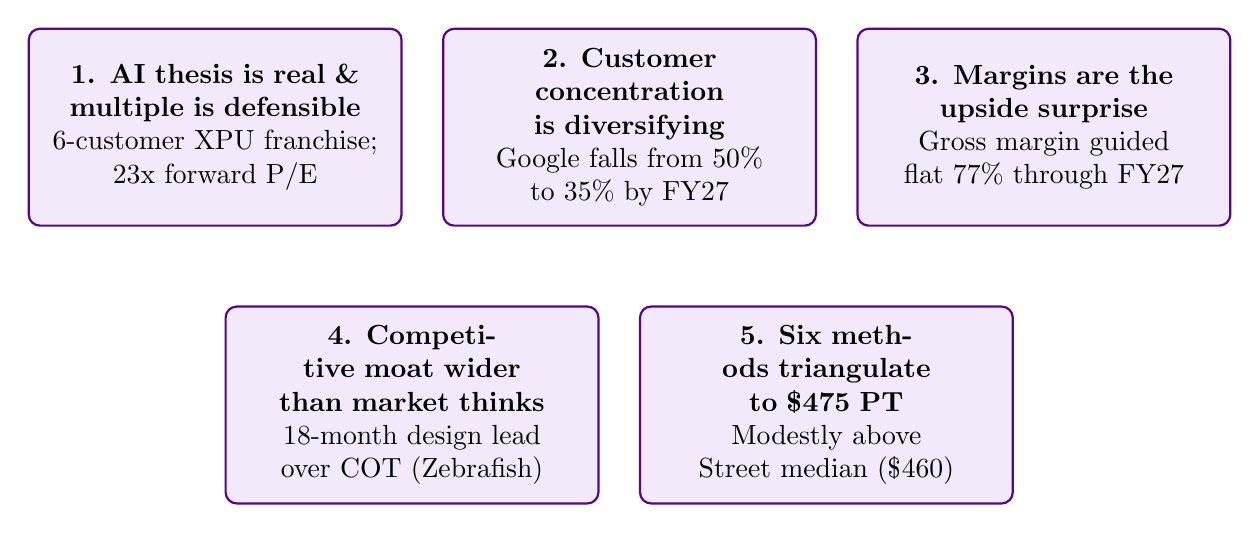
\begin{tikzpicture}[
    box/.style={draw=nyuviolet, thick, fill=rowshade, rounded corners, align=center, text width=4.5cm, minimum height=2.5cm},
    node distance=0.5cm and 0.5cm
  ]
    
    \node[box] (box1) {\textbf{1. AI thesis is real \&}\\ \textbf{multiple is defensible}\\ 6-customer XPU franchise; \\23x forward P/E};
    \node[box, right=of box1] (box2) {\textbf{2. Customer concentration}\\ \textbf{is diversifying}\\ Google falls from 50\% \\to 35\% by FY27};
    \node[box, right=of box2] (box3) {\textbf{3. Margins are the}\\ \textbf{upside surprise}\\ Gross margin guided\\flat 77\% through FY27};
    
    \node[box, below=1cm of box1, xshift=2.5cm] (box4) {\textbf{4. Competitive moat wider}\\ \textbf{than market thinks}\\ 18-month design lead \\over COT (Zebrafish)};
    \node[box, right=of box4] (box5) {\textbf{5. Six methods triangulate}\\ \textbf{to \$475 PT}\\ Modestly above \\Street median (\$460)};
    
  \end{tikzpicture}
  \end{center}
\end{frame}

% =============================================================================
% SLIDE 3: Business overview
% =============================================================================
\begin{frame}{Business Overview: Two Segments, One Model}
  \begin{columns}[T]
    \begin{column}{0.48\textwidth}
      \vspace{0.5cm}
      
\begin{tikzpicture}
        \node[fill=nyuviolet, text=white, rounded corners, minimum width=\textwidth, minimum height=0.8cm, align=center] {\textbf{Semiconductor Solutions}};
      \end{tikzpicture}
      \begin{itemize}
        \item \textbf{Scale:} \$40.0B (62\% of FY25 Rev)
        \item \textbf{Products:} Custom AI accelerators (XPUs), networking silicon, wireless, broadband, storage.
        \item \textbf{AI Shift:} Cyclical legacy business transformed by \$24B annualized AI run-rate (growing 100\%+ YoY).
      \end{itemize}
    \end{column}
    \begin{column}{0.48\textwidth}
      \vspace{0.5cm}
      
\begin{tikzpicture}
        \node[fill=nyudark, text=white, rounded corners, minimum width=\textwidth, minimum height=0.8cm, align=center] {\textbf{Infrastructure Software}};
      \end{tikzpicture}
      \begin{itemize}
        \item \textbf{Scale:} \$23.9B (38\% of FY25 Rev)
        \item \textbf{Products:} VMware Cloud Foundation, Symantec, CA mainframe.
        \item \textbf{Economics:} 92\%+ gross margin subscription model.
      \end{itemize}
    \end{column}
  \end{columns}
  
  \vspace{0.8cm}
  \begin{center}
    \small\textbf{The Broadcom Playbook (Hock Tan, CEO since 2006):}\\
    Serial M\&A $\rightarrow$ Strip overhead $\rightarrow$ Re-price to top enterprises. (5Y Rev CAGR: 23.5\%)
  \end{center}
\end{frame}

% =============================================================================
% SLIDE 4: What changed: the AI customer story
% =============================================================================
\begin{frame}{What Changed: The AI Customer Story}
  \begin{columns}[T]
    \begin{column}{0.4\textwidth}
      \vspace{0.5cm}
      \textbf{Six Committed XPU Customers:}
      \begin{itemize}
          \item \textbf{Google (TPU):} The anchor program (\$27B $\rightarrow$ \$35B in FY27).
          \item \textbf{Anthropic:} Explodes to \$42B in FY27 via Google Cloud (largest contributor).
          \item \textbf{Meta (MTIA):} Extended through 2029 (multi-GW).
          \item \textbf{OpenAI:} 10-GW co-design deal (\$3B $\rightarrow$ \$10B).
      \end{itemize}
      \vspace{0.3cm}
      Management's FY27 ``\$100B+'' AI revenue guide is fully supported by the XPU portfolio effect.
    \end{column}
    \begin{column}{0.6\textwidth}
      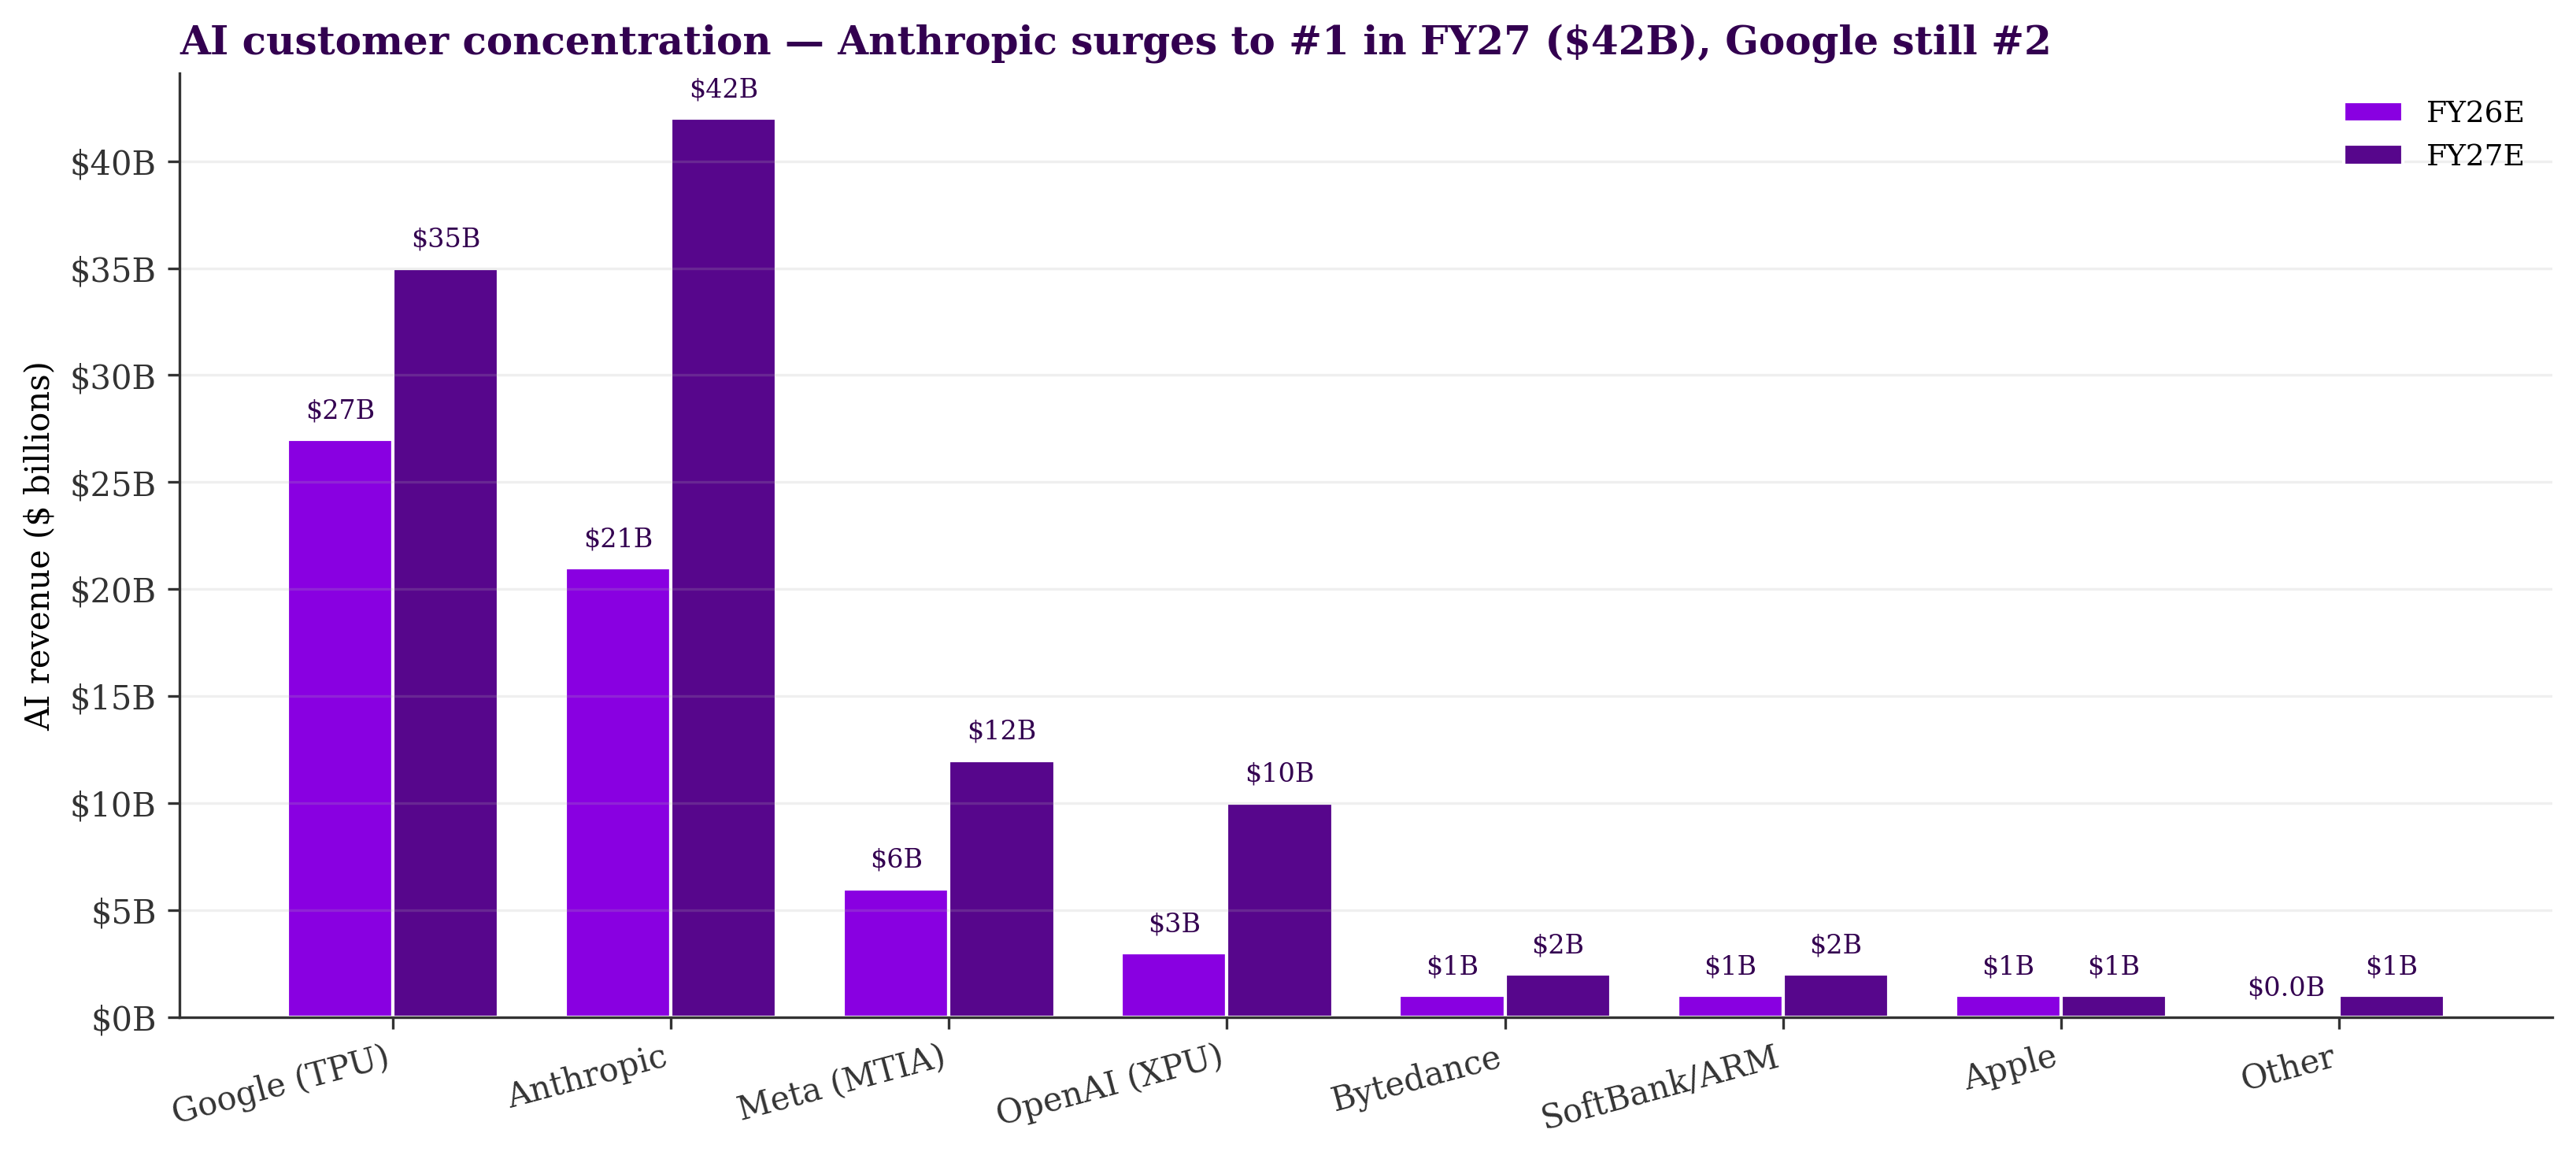
\includegraphics[width=\textwidth,height=5.5cm,keepaspectratio]{fig8_ai_customers.png}
    \end{column}
  \end{columns}
\end{frame}

% =============================================================================
% SLIDE 5: Recent strategic catalysts
% =============================================================================
\begin{frame}{Recent Strategic Catalysts}
  \begin{center}
    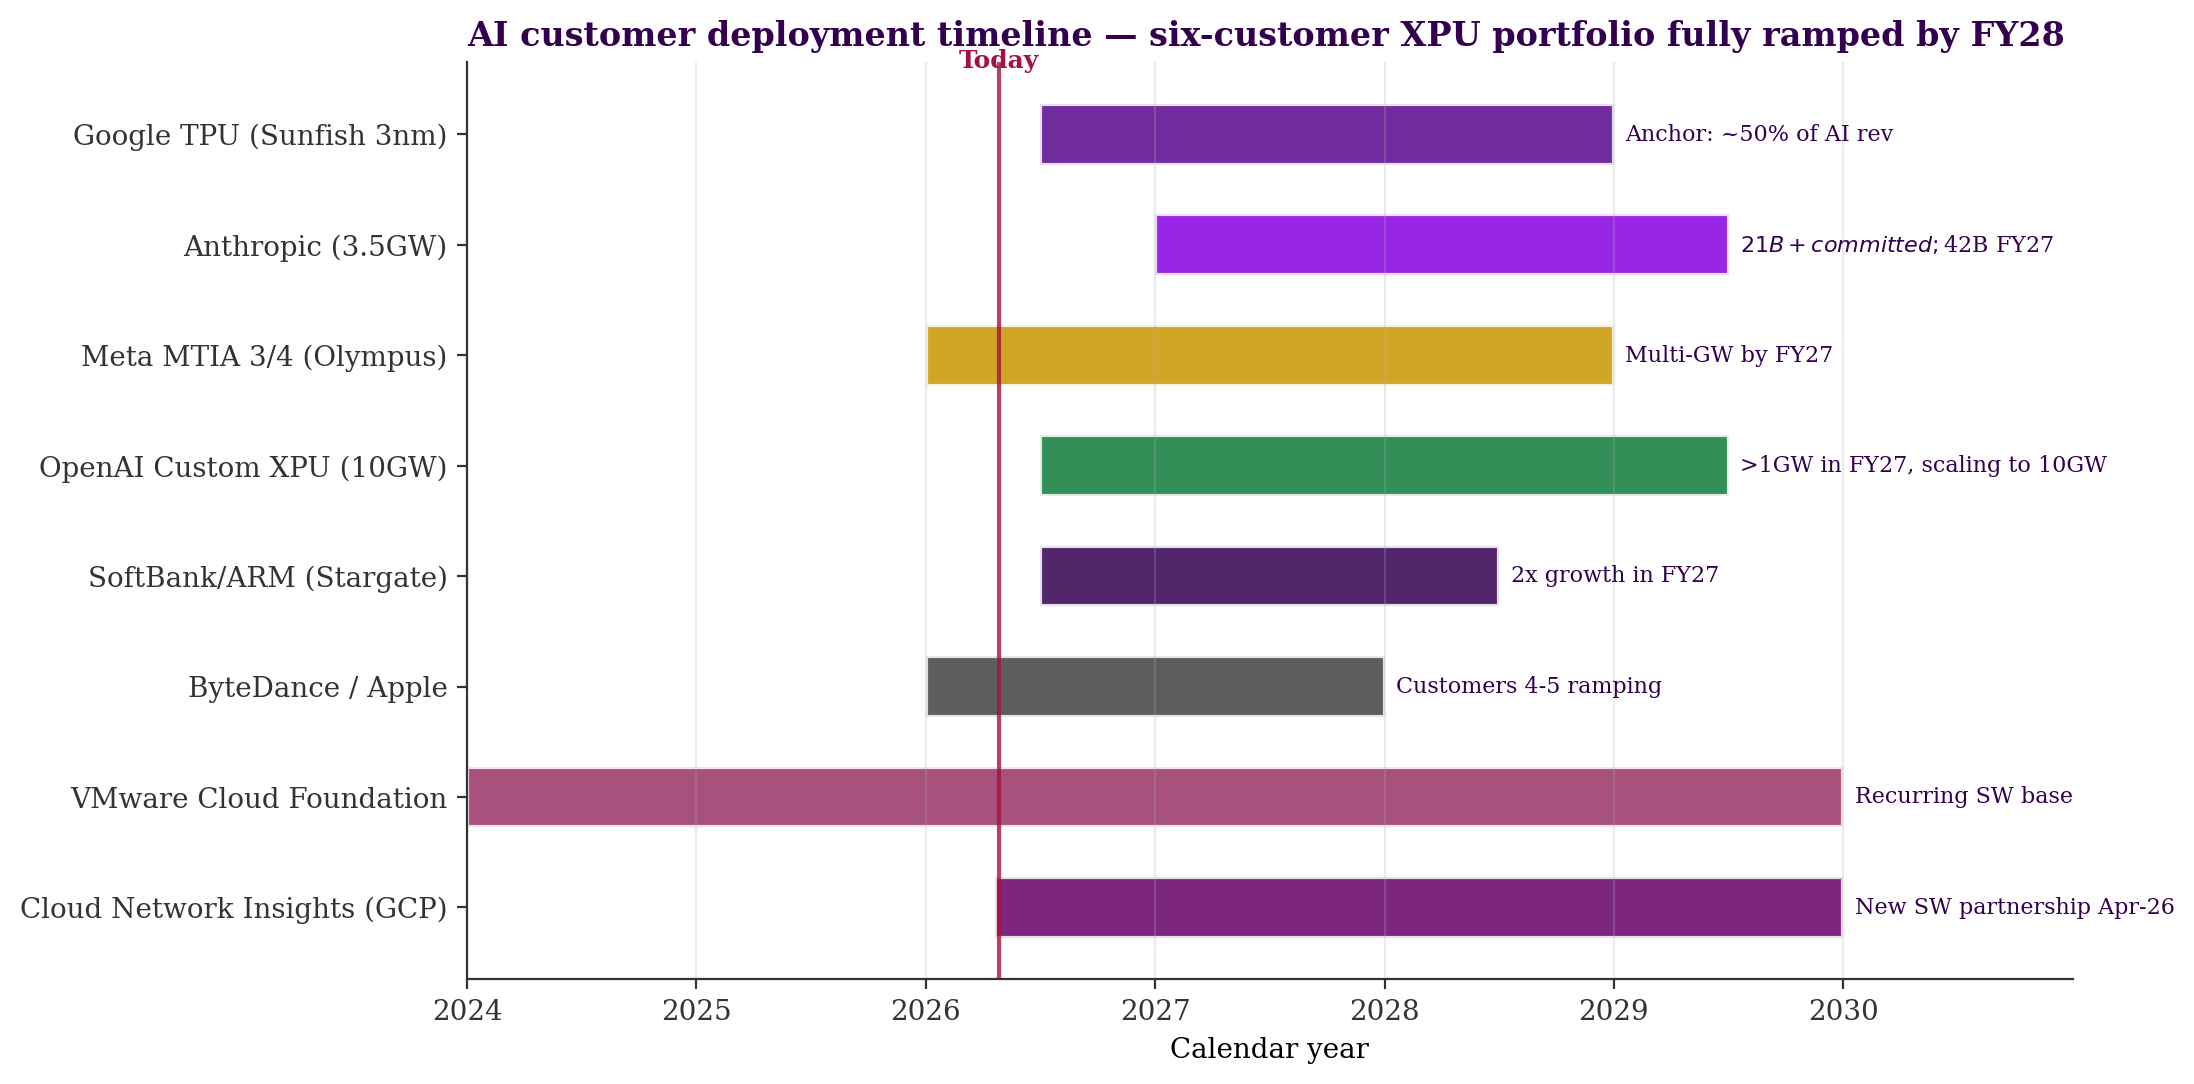
\includegraphics[width=0.95\textwidth]{fig9_deal_timeline.png}
  \end{center}
  \vspace{-0.2cm}
  \begin{itemize}
      \item \textbf{Oct 2025:} OpenAI 10-GW custom XPU partnership (Customer 6).
      \item \textbf{Apr 2026:} Anthropic 3.5-GW 3-way deal via Google Cloud.
      \item \textbf{Apr 2026:} Meta MTIA extended through 2029.
  \end{itemize}
  \small\textit{Catalysts pushed AVGO into the \$2T club. 8 of 11 covering analysts still see upside.}
\end{frame}

% =============================================================================
% SLIDE 6: Financial trajectory
% =============================================================================
\begin{frame}{Financial Trajectory}
  \begin{columns}[T]
    \begin{column}{0.5\textwidth}
      \vspace{0.5cm}
      \textbf{Top-Line Growth (41\% AI CAGR)}
      \begin{itemize}
          \item \textbf{FY26E:} \$105B (+64\% YoY)
          \item \textbf{FY27E:} \$163B
          \item \textbf{FY30E:} \$292B
      \end{itemize}
      \vspace{0.3cm}
      \textbf{Margin Expansion}
      \begin{itemize}
          \item EBITDA expands from 67.7\% today to 72\% by FY30.
          \item Reversal of rack-scale margin warning was the largest Q1 positive surprise.
      \end{itemize}
    \end{column}
    \begin{column}{0.5\textwidth}
      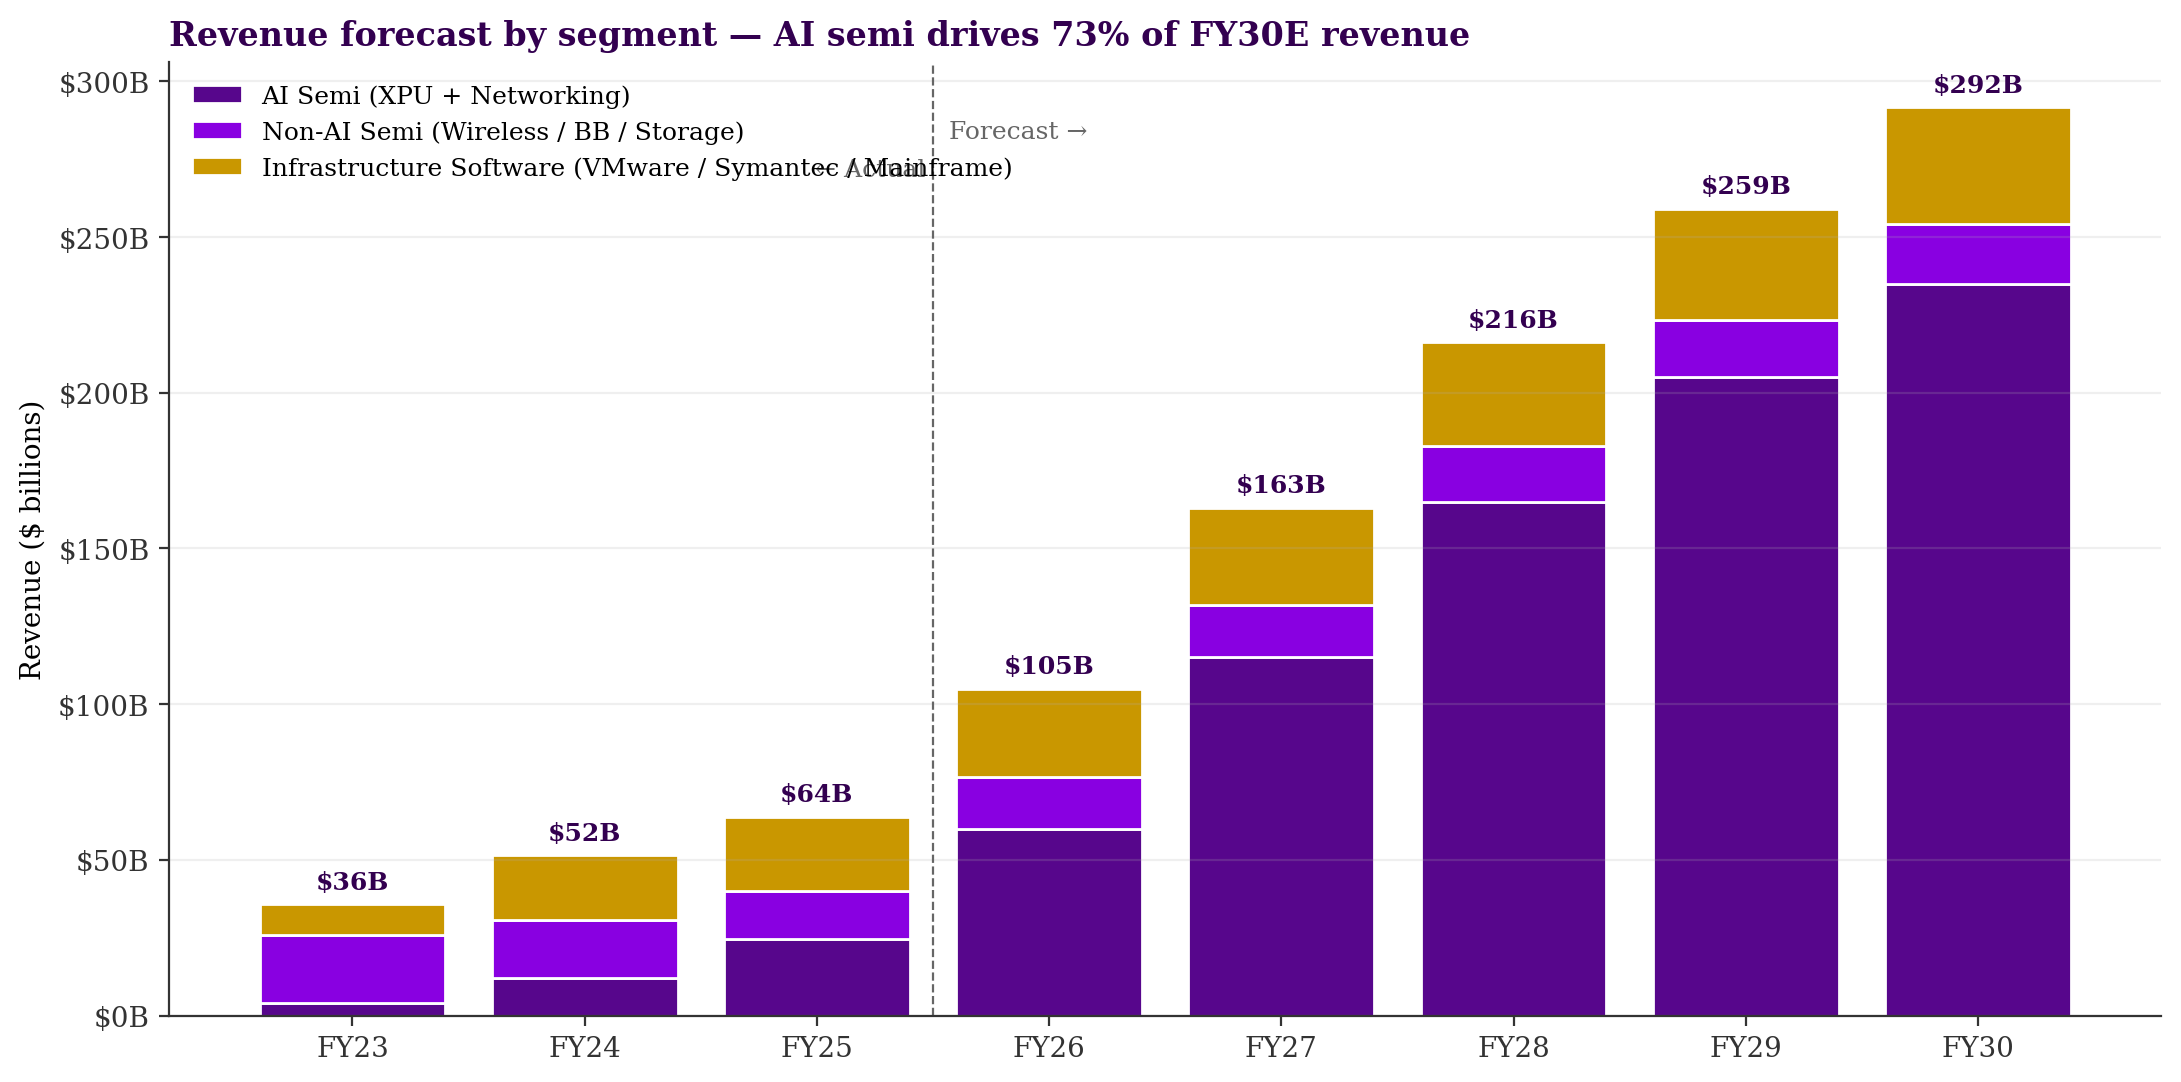
\includegraphics[width=\textwidth,height=5.5cm,keepaspectratio]{fig2_revenue_bridge.png}
    \end{column}
  \end{columns}
\end{frame}

% =============================================================================
% SLIDE 7: Valuation framework overview
% =============================================================================
\begin{frame}{Valuation Framework}
  \begin{center}
  \vspace{1cm}
  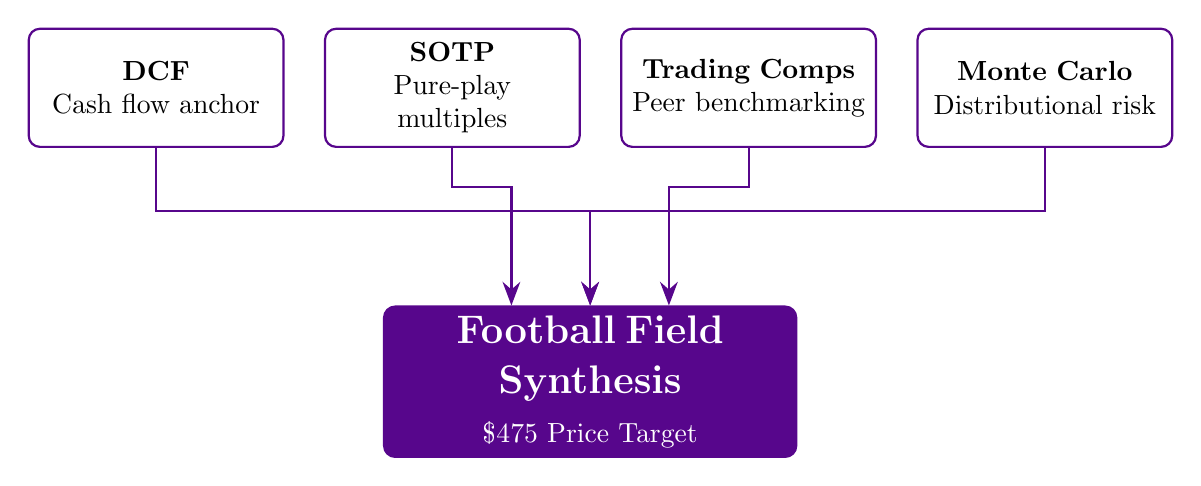
\begin{tikzpicture}[
    box/.style={draw=nyuviolet, thick, fill=white, rounded corners, align=center, text width=3cm, minimum height=1.5cm},
    arrow/.style={-{Stealth[length=3mm]}, thick, nyuviolet}
  ]
    
    \node[box] (dcf) {\textbf{DCF}\\Cash flow anchor};
    \node[box, right=0.5cm of dcf] (sotp) {\textbf{SOTP}\\Pure-play multiples};
    \node[box, right=0.5cm of sotp] (comps) {\textbf{Trading Comps}\\Peer benchmarking};
    \node[box, right=0.5cm of comps] (mc) {\textbf{Monte Carlo}\\Distributional risk};
    
    \node[box, fill=nyuviolet, text=white, text width=5cm, below=2cm of sotp, xshift=1.75cm] (ff) {\Large\textbf{Football Field Synthesis}\\[0.2cm]\normalsize \$475 Price Target};
    
    \draw[arrow] (dcf.south) -- ++(0,-0.8) -| (ff.north);
    \draw[arrow] (sotp.south) -- ++(0,-0.5) -| ([xshift=-1cm]ff.north);
    \draw[arrow] (comps.south) -- ++(0,-0.5) -| ([xshift=1cm]ff.north);
    \draw[arrow] (mc.south) -- ++(0,-0.8) -| (ff.north);
    
  \end{tikzpicture}
  \vspace{0.5cm}
  
  \textit{The intersection of independent methods yields a defensible fair-value range.}
  \end{center}
\end{frame}

% =============================================================================
% SLIDE 8: DCF
% =============================================================================
\begin{frame}{Discounted Cash Flow (DCF)}
  \begin{columns}[T]
    \begin{column}{0.4\textwidth}
      \vspace{0.5cm}
      \textbf{WACC Build (9.50\%)}
      \begin{itemize}
          \item \textbf{Rf:} 4.31\% (10Y T-Note)
          \item \textbf{ERP:} 5.0\%
          \item \textbf{Beta:} 1.20 (2Y weekly)
          \item \textbf{Cost of Debt:} 5.0\% (pre-tax)
          \item \textbf{Terminal Growth:} 3.0\%
      \end{itemize}
      \vspace{0.5cm}
      \textbf{Result}
      \begin{itemize}
          \item \textbf{Base Case:} \$436 per share.
          \item \textbf{Sensitivity:} \$402--\$474 range at $\pm$50bps WACC.
          \item \textit{Caveat: Terminal value is 80\% of EV.}
      \end{itemize}
    \end{column}
    \begin{column}{0.6\textwidth}
      \vspace{-0.2cm}
      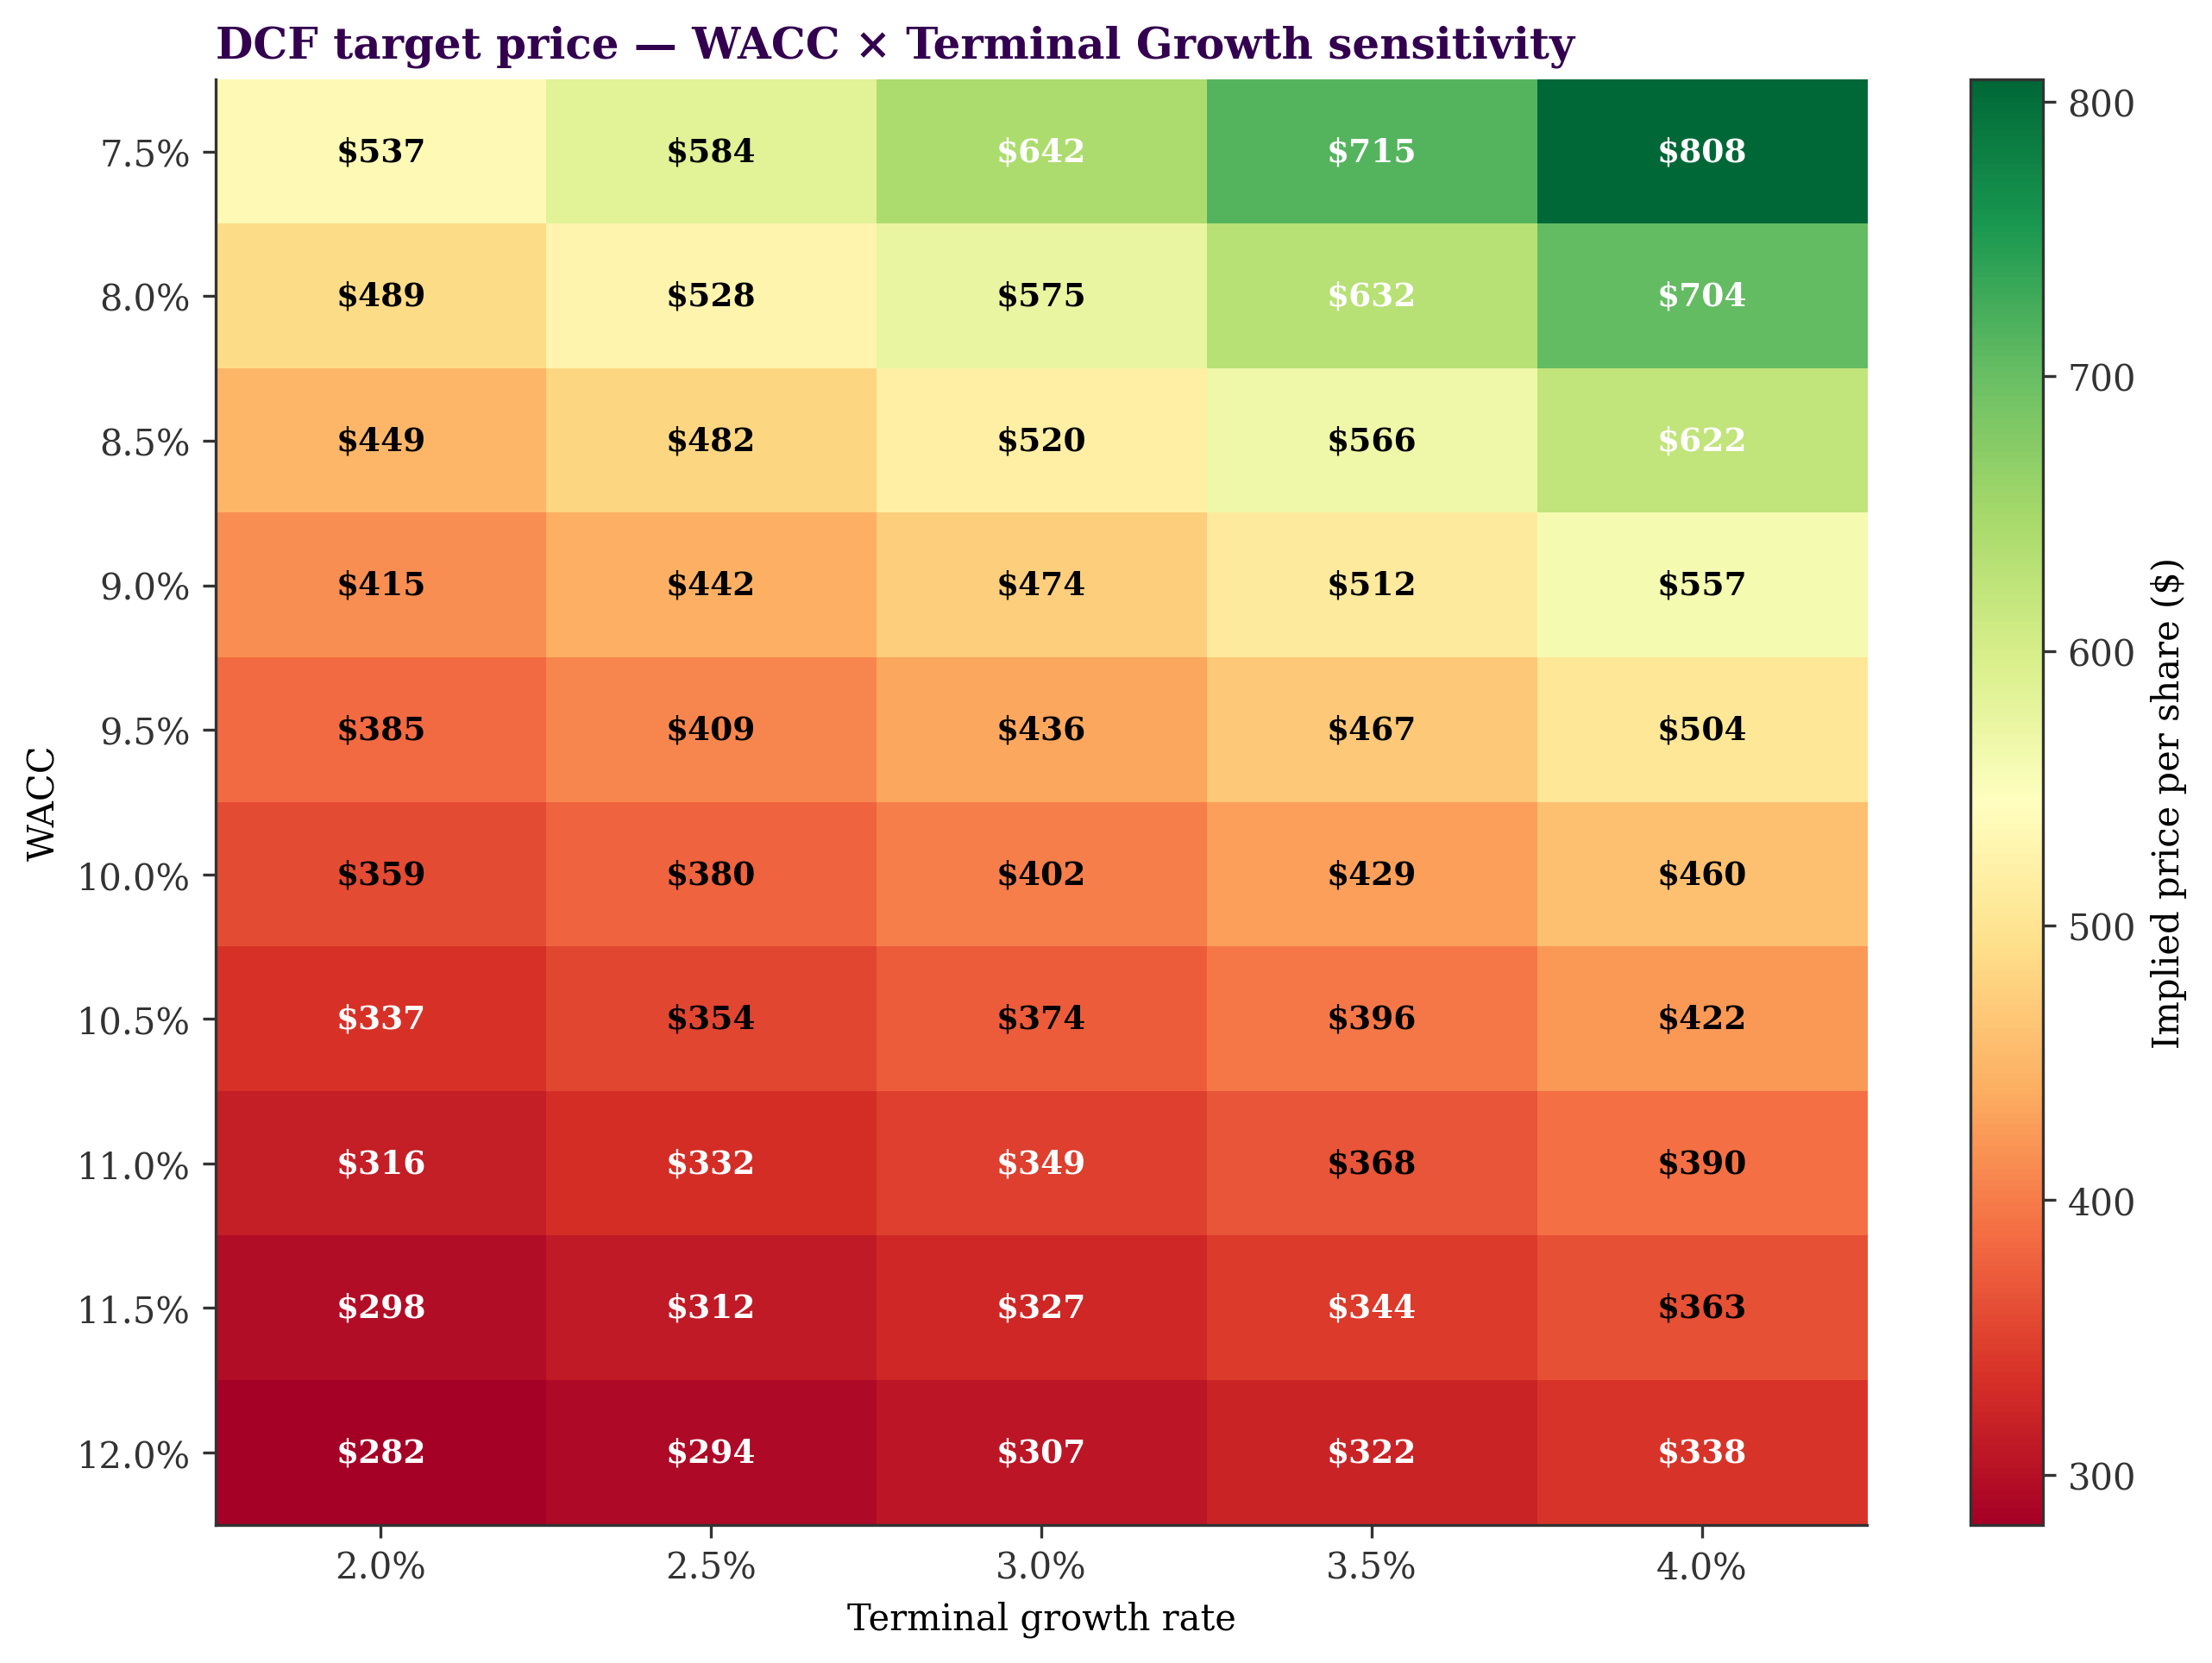
\includegraphics[width=\textwidth]{fig6_sensitivity.png}
    \end{column}
  \end{columns}
\end{frame}

% =============================================================================
% SLIDE 9: SOTP & Comps
% =============================================================================
\begin{frame}{Sum-of-the-Parts \& Trading Comparables}
  \begin{columns}[T]
    \begin{column}{0.5\textwidth}
      \textbf{Sum-of-the-Parts (Mid: \$401)}
      \vspace{0.2cm}
      
      \small
      \begin{tabularx}{\textwidth}{@{}X r r@{}}
        \toprule
        \textbf{Segment} & \textbf{Mult} & \textbf{Val (\$)} \\
        \midrule
        Semi (EBITDA 62\%) & 20x & \$321 \\
        Software (EBITDA 77\%) & 17x & \$482 \\
        \midrule
        \textbf{Implied Price} & & \textbf{\$401} \\
        \bottomrule
      \end{tabularx}
      \vspace{0.4cm}
      \begin{itemize}
          \item Separates hardware (NVIDIA/AMD comps) from mature SaaS.
      \end{itemize}
    \end{column}
    \begin{column}{0.5\textwidth}
      \textbf{Trading Comps (Fwd P/E Mid: \$414)}
      \vspace{0.2cm}
      
      \small
      \begin{tabularx}{\textwidth}{@{}X r r@{}}
        \toprule
        \textbf{Multiple} & \textbf{Ratio} & \textbf{Val (\$)} \\
        \midrule
        Fwd P/E (on \$18.83) & 22x & \$414 \\
        EV/EBITDA & 18x & \$409 \\
        \bottomrule
      \end{tabularx}
      \vspace{0.4cm}
      \begin{itemize}
          \item Peer median Fwd P/E is 28.3x; we apply a conservative 22x.
          \item Peer median EV/EBITDA skewed by AMD/MRVL (31.8x).
      \end{itemize}
    \end{column}
  \end{columns}
  \vspace{0.8cm}
  \begin{center}
      \textit{Both relative methods cluster between \$400 and \$440, supporting the DCF base case.}
  \end{center}
\end{frame}

% =============================================================================
% SLIDE 10: Monte Carlo
% =============================================================================
\begin{frame}{Monte Carlo Simulation}
  \begin{columns}[T]
    \begin{column}{0.4\textwidth}
      \textbf{10,000 Paths | 6 Inputs}
      \begin{itemize}
          \item \textbf{FY27 AI Rev:} Normal(\$125B, \$25B) - Anchors on Street median.
          \item \textbf{Terminal g:} Normal(3.0\%, 0.5\%)
          \item \textbf{WACC:} Normal(9.5\%, 0.5\%)
      \end{itemize}
      \vspace{0.3cm}
      \textbf{Result}
      \begin{itemize}
          \item \textbf{Mean:} \$471
          \item \textbf{P25 / P75:} \$378 / \$544
          \item \textbf{Probability $>$ Spot:} \textbf{68.3\%}
      \end{itemize}
    \end{column}
    \begin{column}{0.6\textwidth}
      \vspace{-0.5cm}
      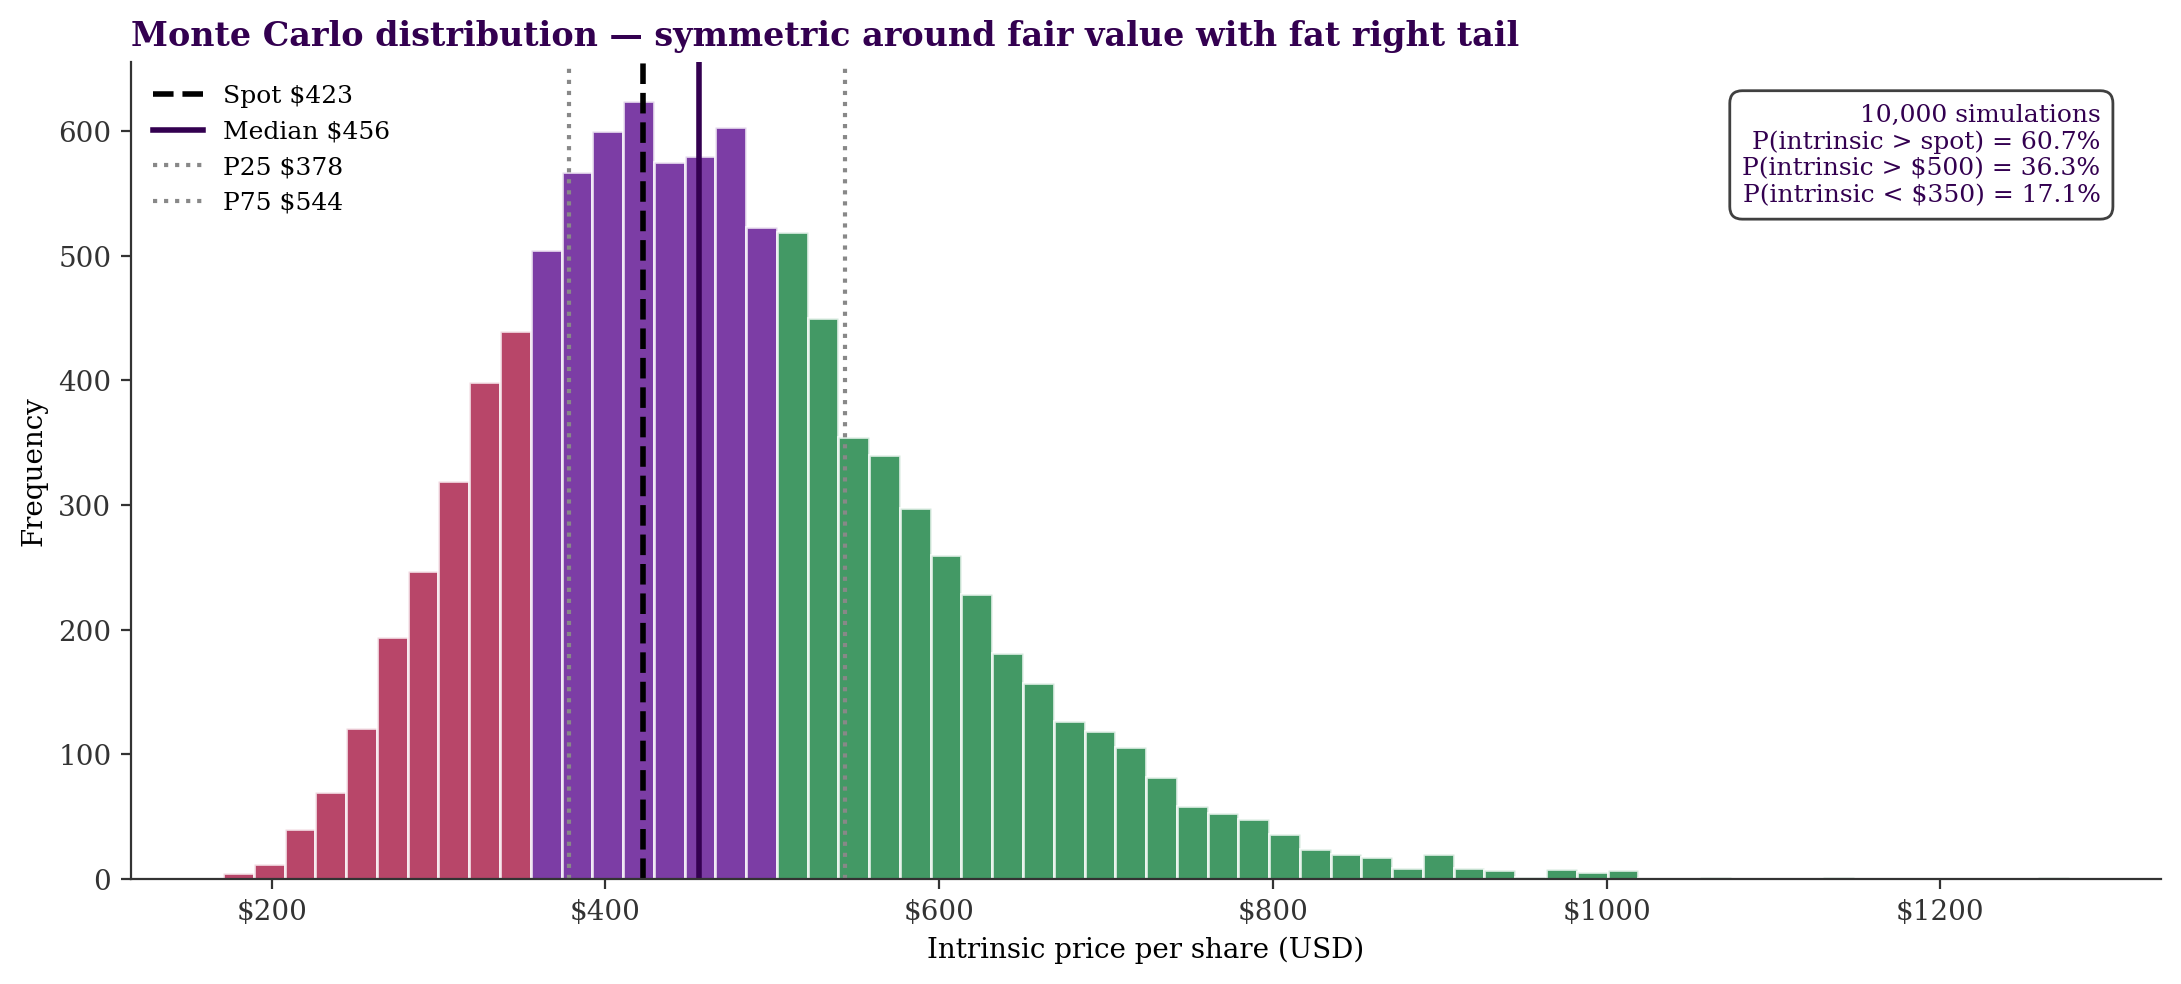
\includegraphics[width=\textwidth,height=5.5cm,keepaspectratio]{fig5_monte_carlo.png}
    \end{column}
  \end{columns}
\end{frame}

% =============================================================================
% SLIDE 11: Football field synthesis
% =============================================================================
\begin{frame}{Football Field Synthesis}
  \begin{center}
    \vspace{-0.2cm}
    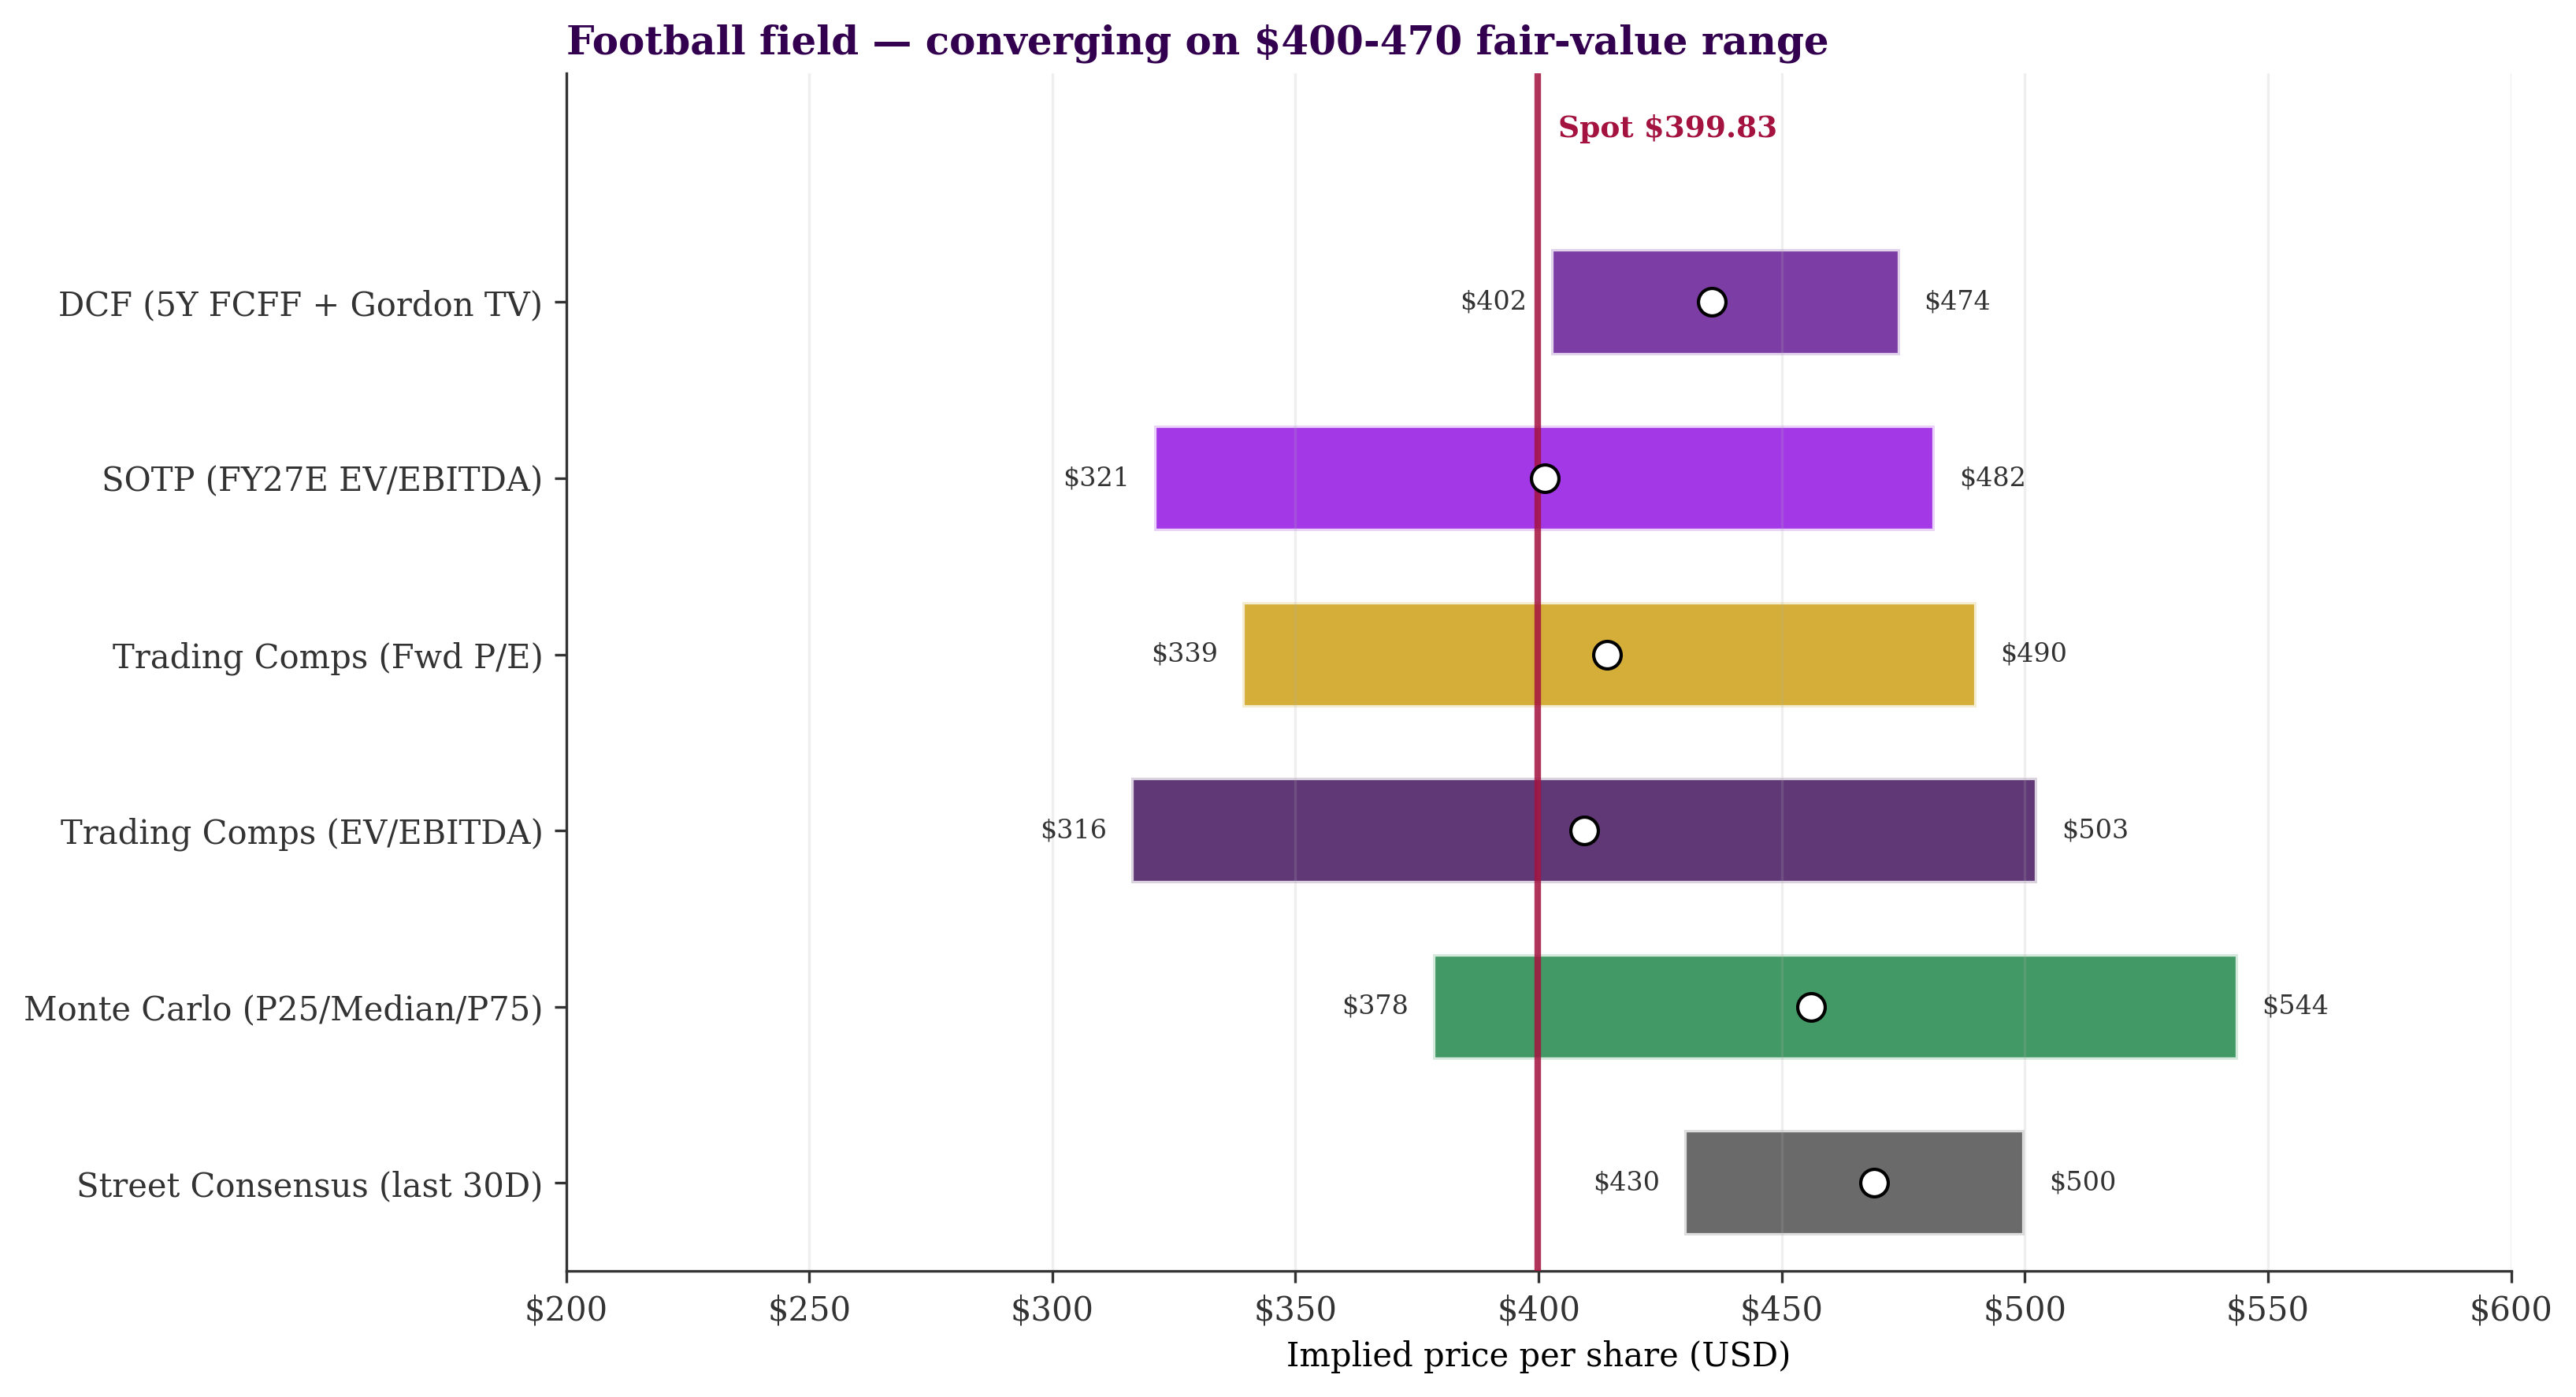
\includegraphics[width=0.9\textwidth]{fig4_football_field.png}
  \end{center}
  \vspace{-0.2cm}
  \begin{itemize}
      \item \textbf{Ranges:} DCF \$402--474, SOTP \$321--482, Comps Fwd P/E \$339--490.
      \item \textbf{Convergence:} Six methods cluster in the \$400--\$510 range.
      \item \textbf{Conclusion:} \$475 PT anchors on the Monte Carlo mean (\$471) plus right-tail premium.
  \end{itemize}
\end{frame}

% =============================================================================
% SLIDE 12: Risk framework
% =============================================================================
\begin{frame}{Risk Framework}
  \begin{columns}[T]
    \begin{column}{0.45\textwidth}
      \vspace{0.3cm}
      \textbf{Top-Right Risks (High Prob/Impact)}
      \begin{itemize}
          \item \textbf{Hyperscaler Capex:} Coordinated Google/Meta/MSFT pullback compresses multiple and revenue (30\% downside modeled).
          \item \textbf{Customer Concentration:} Google + Anthropic $\sim$60\% of FY27 AI mix.
          \item \textbf{AI Bubble Revaluation:} AVGO highly exposed to multiple compression given 80\% terminal value share.
      \end{itemize}
    \end{column}
    \begin{column}{0.55\textwidth}
      \vspace{-0.5cm}
      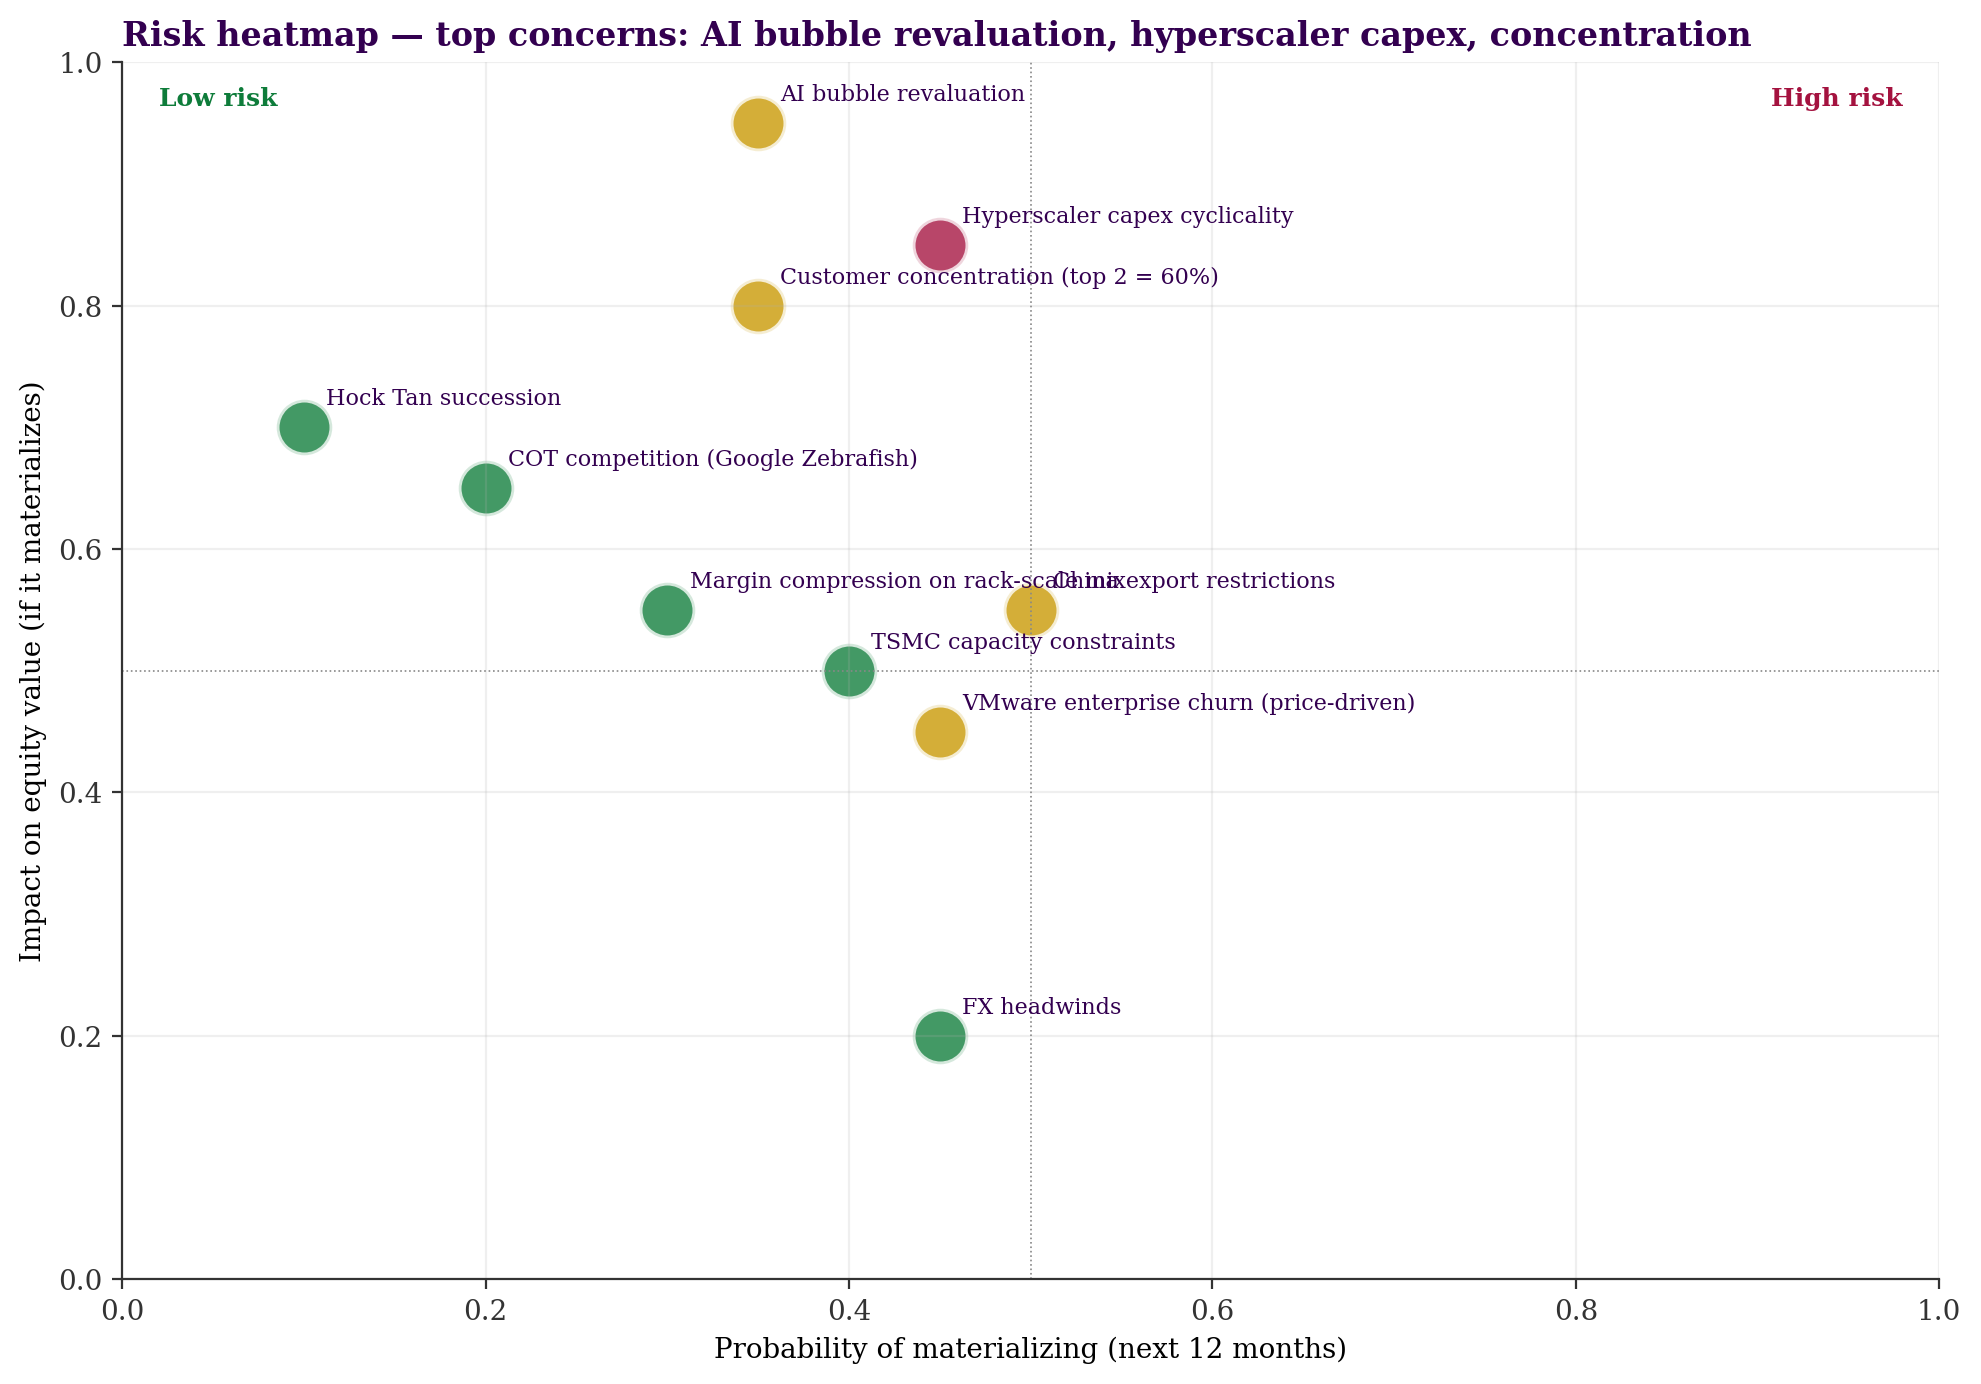
\includegraphics[width=\textwidth,height=5.5cm,keepaspectratio]{fig11_risk_matrix.png}
    \end{column}
  \end{columns}
\end{frame}

% =============================================================================
% SLIDE 13: Catalyst calendar
% =============================================================================
\begin{frame}{Catalyst Calendar \& What Would Change Our View}
  \vspace{0.5cm}
  \renewcommand{\arraystretch}{1.5}
  \begin{tabularx}{\textwidth}{@{}l X@{}}
    \toprule
    \textbf{Date} & \textbf{Catalyst Event} \\
    \midrule
    \textbf{5-Jun-2026} & Q2 earnings — AI revenue actuals vs. \$10.7B guide. \\
    \rowcolor{rowshade}\textbf{H2-2026} & TPU Sunfish 3nm volume ramp + OpenAI rack deployments. \\
    \textbf{4-Sep-2026} & Q3 earnings — First framing commentary on FY27. \\
    \rowcolor{rowshade}\textbf{Dec-2026} & Q4 + FY27 Guide — Critical print to validate \$100B+ AI floor. \\
    \bottomrule
  \end{tabularx}
  
  \vspace{0.8cm}
  \begin{center}
  
\begin{tikzpicture}
    \node[draw=accentred, thick, fill=white, rounded corners, inner sep=0.3cm, text width=10cm, align=center] {
        \textbf{\color{accentred}What would move us off BUY:}\\
        Spot breaks \$475 \textbar{} FY27 AI guide $<$ \$100B \textbar{} Google share-loss to Zebrafish
    };
  \end{tikzpicture}
  \end{center}
\end{frame}

% =============================================================================
% SLIDE 14: Recommendation summary
% =============================================================================
\begin{frame}[plain]
  \begin{tikzpicture}[remember picture,overlay]
    \fill[white] (current page.south west) rectangle (current page.north east);
    \fill[nyuviolet] ([yshift=-1.5cm]current page.north west) rectangle (current page.north east);
    
    \node[anchor=center, text=white] at ([yshift=-0.75cm]current page.north) {\Huge\textbf{Recommendation Summary}};
    
    \node[anchor=center, align=center] at ([yshift=0.5cm]current page.center) {
        \Huge\textbf{Broadcom Inc. (AVGO)}\\[0.5cm]
        \begin{tikzpicture}
            \node[fill=accentgreen, text=white, minimum width=8cm, minimum height=1.5cm, rounded corners] {\Huge\textbf{BUY \textbar{} \$475 PT \textbar{} +19\%}};
        \end{tikzpicture}\\[0.5cm]
        \Large\textbf{68.3\% probability of upside vs. \$399.83 spot}\\[0.3cm]
        \normalsize Top Catalyst: Dec-2026 FY27 Guide \textbar{} Top Risk: Hyperscaler Capex
    };
    
    \node[anchor=south, text=nyugrey, align=center] at ([yshift=1cm]current page.south) {
        \textbf{Q\&A}\\[0.2cm]
        Tanishk Yadav \textbar{} Martin Baretto \textbar{} Ramana Sriram
    };
  \end{tikzpicture}
\end{frame}

\end{document}
